\chapter{Data Processing}\label{ch:2}
\epigraph{On two occasions I have been asked, ""'Pray, Mr. Babbage, if you put into the machine wrong figures, will the right answers come out?'"" ... I am not able rightly to apprehend the kind of confusion of ideas that could provoke such a question.}{Charles Babbage}

The goal of data mining can be defined as the process of obtaining knowledge from underlying data by systematic using of analytic methods on it. In this thesis we are up to obtain anomalies in data and the analytic methods are the machine learning algorithms discussed in Chapter~\ref{ch:3}. 

However, data-mining is more than applying algorithms on data. Extracting valuable results efforts among other things the consideration of a basis principle in the field of computer science known as \textit{Garbage In Garbage Out (GIGO)}. The business dictionary \footnote{http://www.businessdictionary.com/definition/garbage-in-garbage-out-GIGO.html}  defines \textit{GIGO} as an axiom used in context of computer science that signifying that no matter how sophisticated an information processing system is, the quality (accuracy, completeness, relevance, timeliness, etc) of the information coming out of it cannot be better than the quality of the information that went in. A program working on inaccurate data will only yield misleading results. The preparation of data has thus a significant contribution to the success of a data-mining goal.

There are several industry established standards like \textit{KDD, SEMMA, CRISP} \footnote{See the work of \cite{Azevedo;Santos;Filipe:2008}.} to name a few, invented to structure a data-mining process. In this thesis we follow the \textit{Cross-industry process for data mining (CRISP-DM)} \cite{crisp} which is a proved data-mining process approach described in terms of an hierarchical process model.
\begin{figure}[h!]
    \centering
    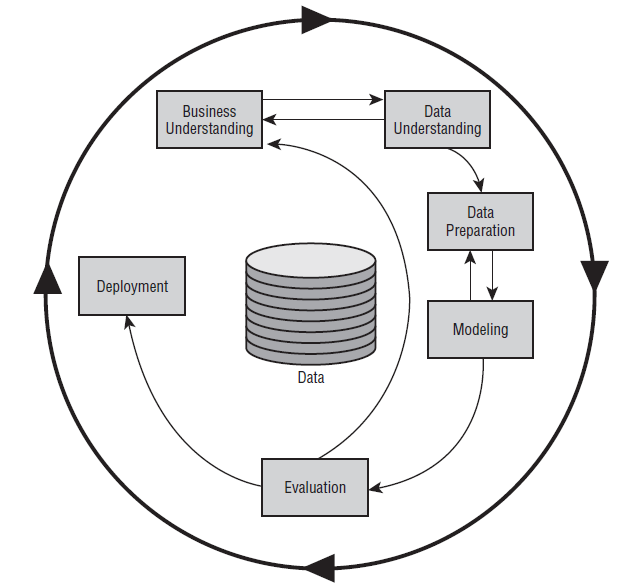
\includegraphics[scale=0.5]{Graphics/crisp-dm.png}
    \caption{CRISP-DM process}
    \label{fig:crisp-dm}
\end{figure}

Here, the CRISP-DM process is a cycle, what implies incremental retrying of particular processes for the sake of improving. However, this chapter will treat only the first three phases of CRISP-DM without the back steps. The goal is to describe the possible operations and their occurring limitations, the practical application of these and the possible back steps will be the content of chapter \ref{Chapter:5}.

This chapter will first provide a macro view of a loan application process to point out the steps our data will come from.

Then, the first three phases of CRISP-DM process are described with respect to the context of this thesis:
\begin{itemize}
    \item \textbf{Business Understanding }  
    \begin{itemize}
        \item Data acquisition (section~\ref{Ch:2:Acquisition}). 
        % DATA Centered Approach, - Data driven
        \item Dataset overview (section~\ref{Ch:2:Overview}) -- a macro view of the entire dataset.
    \end{itemize}
    \item \textbf{Data Understanding }
        \begin{itemize}
            \item Feature description~(section~\ref{Ch:2:FeatureDesc}) -- a micro view of feature characteristics and type.
            \item Data exploration (section~\ref{Ch:2:Exploration}) -- statistical and visual summaries, data quality, correlated features.
        \end{itemize}
    \item \textbf{Data Preparation }
            \begin{itemize}
                \item Data preprocessing (section~\ref{Ch:2:Preprocessing}) -- preparation for data mining.
        \end{itemize}
\end{itemize}

\section{Data Acquisition}\label{Ch:2:Acquisition}
The underlying data treated in this thesis contain information, collected during the credit enquiry process, briefly illustrated in figure \ref{fig:behav-data}. In course of the application the potential borrower provides his personal information by stepping through a number of steps in the web application form. His/her interactions with web-form elements, such as pressed keys or tracked time between actions, are also collected. Figure~\ref{fig:behav-data}shows an overview of data collecting \footnote{Each step signifies a step that the potential borrower has to accomplish to get a loan. Behavioral features are collected in each of the particular steps. There are three different scopes of behavioral features: scope of particular webpage, scope of webform elements, scope of web-slider (special webform element).}. 

After fetching from an SQL database, the data is represented by a matrix whose rows are loan applications and columns are features associated with each loan application. 

\begin{figure}[h!]
    \centering
    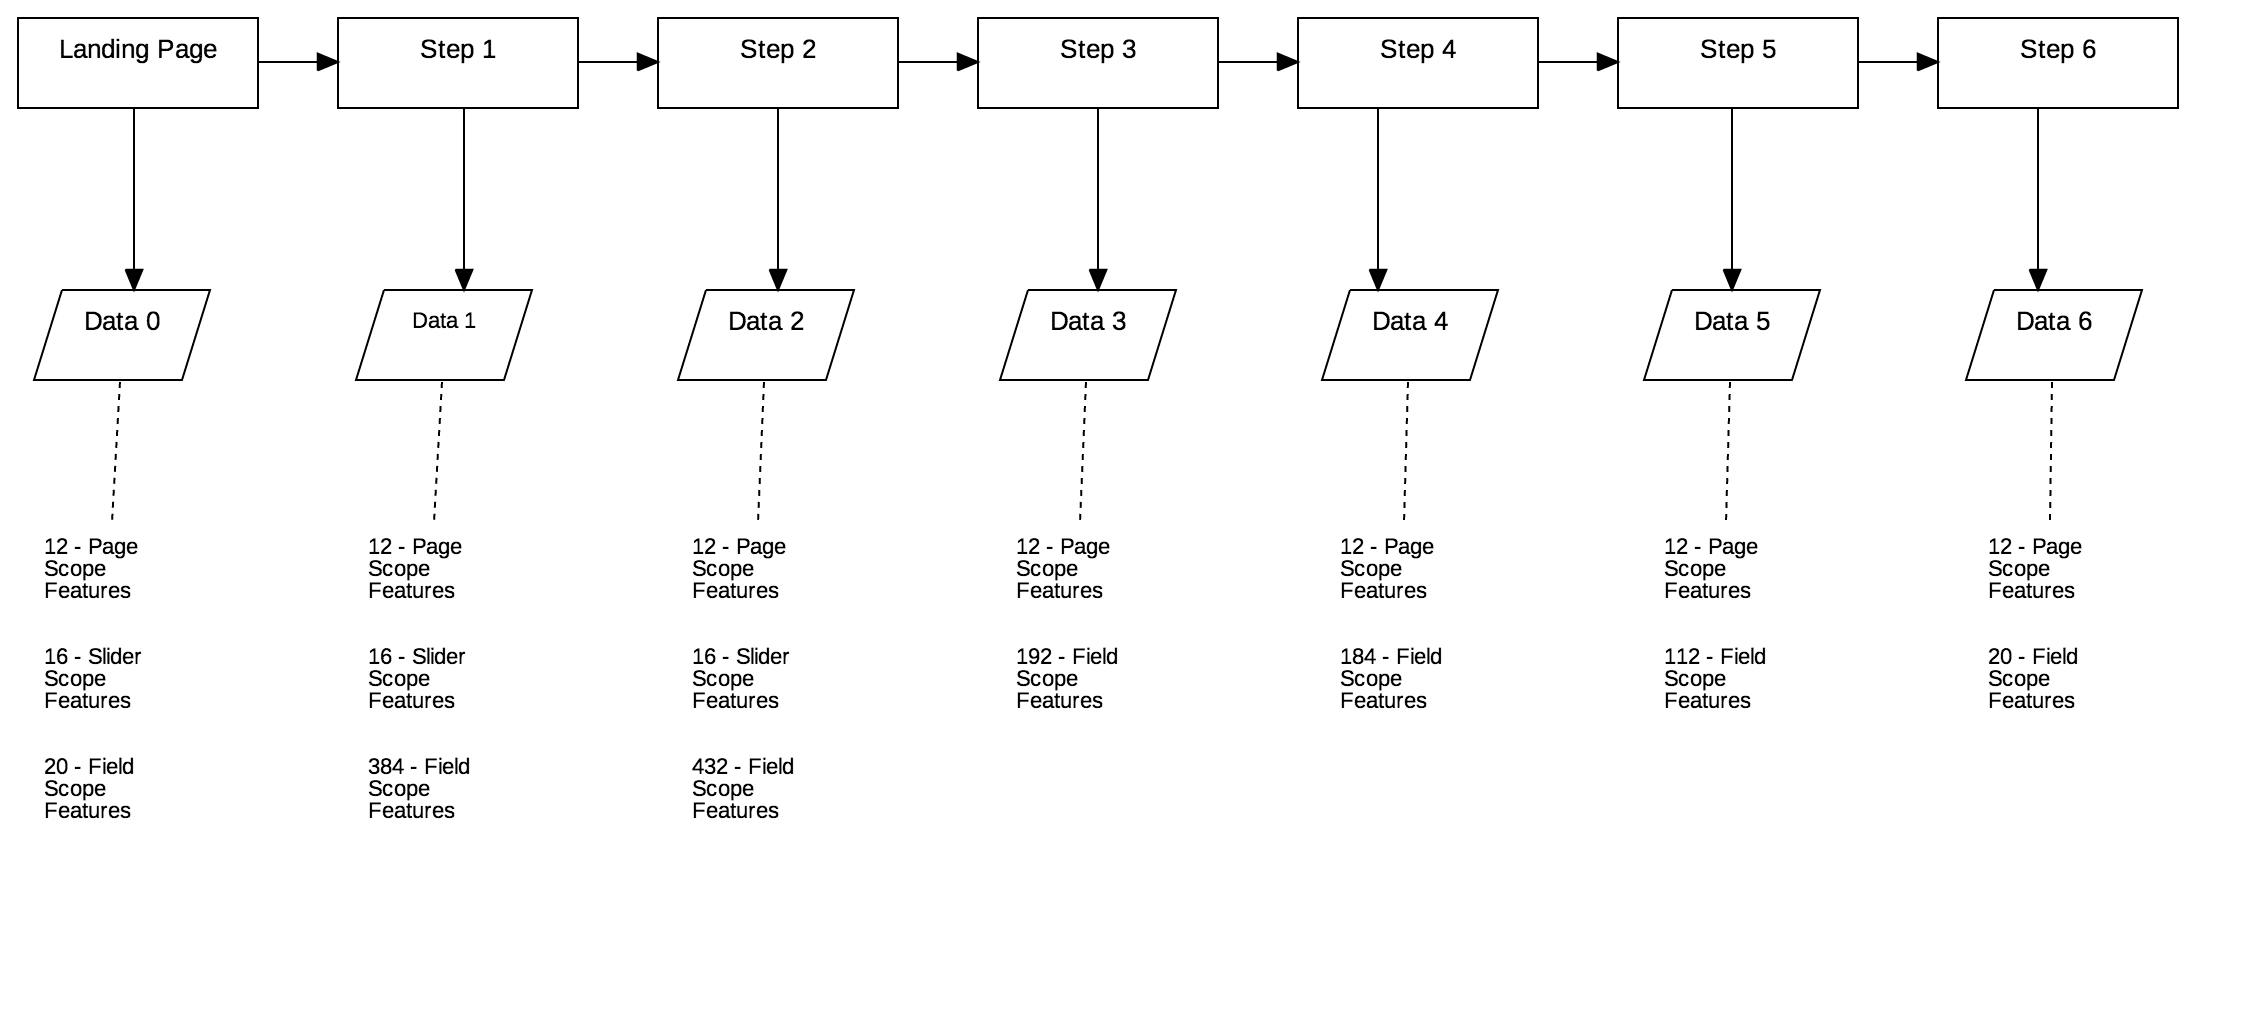
\includegraphics[scale=0.20]{Graphics/FlowchartDiagram1.png}
    \caption{Collection of behavioral data.}
    \label{fig:behav-data}
\end{figure}

The features are either categorical or numeric and come from the two different sources:
\begin{itemize}
    \item Applicant input collected from a loan applicant.
    \item System input collected by an application processing system.
\end{itemize}

User input (data an applicant reports about himself/herself) may be inaccurate (for example, due to mistyping or deliberate attempt of cheating) and therefore it is dismissed from further analysis.
More objective information is deemed to be collected from  applicant's behavior when he/she is filling web forms. Manipulation of behavioral information is significantly more difficult than filling in false personal data.

As fraud intended to bypass a scoring system and get a loan despite of false information is one of the anomalies, behavioral features serve as a basis for anomaly detection. 

\section{Dataset Overview}\label{Ch:2:Overview}
An effective utilization of data requires a profound understanding of available data -- also from a nontechnical perspective.

Each data instance is representing information of an individual credit application, the information is historical and represents a common fact of a granted loan. Granted means that this application have been approved by a scoring algorithm and the loan is issued to a borrower. Identifying anomalies signifying malicious actions in this type of data is of particular interest to prevent fraud in the future.

We introduce three assumptions on the available data for further analysis.

\textbf{Fraud:} 
A small subset hold applications that in retrospect turned out to have fraudulent intention. This can have different causes, a portion has been reported by the local law enforcements, others are results of identity abuse or other malicious actions.

\textbf{Non Fraud:} 
A subset of applications where borrowers have already payed at least one installment back (long-term loan, e.g., issued for one year) or fully repaid a loan (short-term loan, e.g., issued for 30 days) is believed not to have any fraudulent intentions. 
\textbf{Unlabeled:}
A notable subset of applications not labeled as fraud but also not having positive cash flow; thus, this data could not be labeled with absolute certainty.

In total of \(95951\) instances.

\section{Feature Description}\label{Ch:2:FeatureDesc}
The underlying dataset contains in total 1804 features for each loan application (instance). A description of each feature is thus not practical. However, a more consolidated analysis is reported in Table~\ref{tab:feature-summary}. 

\begin{table}[h!]
  \begin{center}
    \caption{Feature type summary}
    \label{tab:feature-summary}
    \begin{tabular}{c|c|c}
    Type & No. of Features & Percentage of the Total \\
      \hline
     Categorical & \(196\) & \(~11\%\) \\ 
     \hline
     Logical & \(90\) &  \(~5\%\) \\
     \hline
     Numeric & \(1519\) &  \(~84\%\) \\
     \hline
    \end{tabular}
  \end{center}
\end{table}

As could be seen, a vast majority of features is numeric, i.e., they can be represented by a number. The examples of numeric features are the number of keys pressed or time to fill a field in the application form. Features that may take only binary values (Yes/No, True/False) are boolean or logical like did an applicant read the term conditions? or did email address given exist?. Features that can be represented by words (or categories) like a city of residence or place of work - are categorical.

Although there are machine learning algorithms that can manage features of different types, a majority requires to convert logical and categorical features into a numeric format. How this is typically done will be explained in~section~\ref{Ch:2:Preprocessing}.

\section{Data Exploration}\label{Ch:2:Exploration}
This task addresses data mining questions by using database querying, visualization, and reporting techniques. These include distributions of key features (for example, target or response), relationships between pairs or small numbers of features, results of simple aggregations, properties of significant subpopulations, and simple statistical analyses. These analyses may directly address the data mining goals, they may also contribute to or refine the data description and quality reports, and feed into the transformation and other data preparation steps needed for further analysis \cite{crisp}.

\subsection{Statistical Summary of Data}\label{Ch:2:SSummary}
In total, our underlying dataset holds 95951 instances of individual applications.

According to the semantic labeling in chapter \ref{Ch:2:Overview}, Table \ref{tab:instance-summary} summarize the amount of particular labels.

\begin{table}[h!]
  \begin{center}
    \caption{Instance Type Summary}
    \label{tab:instance-summary}
    \begin{tabular}{c|c|c}
    Label & No. of Cases & Percentage of the Total \\
      \hline
     Fraud & \(744\) & \(~1\%\) \\ 
     \hline
     Non-fraud & \(8.2525\) &  \(~86\%\) \\
     \hline
     Unlabeled & \(12.682\) &  \(~13\%\) \\
     \hline
    \end{tabular}
  \end{center}
\end{table}

Non-fraudulent instances clearly dominate the dataset while the fraudulent ones constitute a small fraction of the entire dataset. As fraud is a particular case of anomaly, this is not surprising.

For categorical features, a summary is as follows: 
\begin{itemize}
    \item \textbf{Min: } 2 Categories
    \item \textbf{Max: } 6 Categories
    \item \textbf{Mean:} 3 Categories
\end{itemize}

Thus, the maximum number of categorical level is not large.
This observation is important insofar as each category adds a further dimension during the categorical to numerical transformation process (section~\ref{Ch:2:CTNT}).

A cumulative analysis of variance (see Table~ \ref{tab:instance-summary}), showed up a low variance in the major part of the distribution. This is an essential information since low variance features can cause noise which can hurt classification accuracy. 

Considering the summary of means (see Table~\ref{tab:instance-summary}) yield two observations: the high difference between the mean and the 3rd Quartile is an indicator for a skewed distribution (e.g high amount of extreme values), these are also a common cause of  misclassification. Moreover, the fact that the underlying  dataset contains negative numeric values leads to the assumption of possible errors occurred during the data acquisition process \footnote{The assumption was confirmed by consulting the responsible department. However, the details of this problem are out of the scope, thus, it is an engineering problem.}.

\begin{table}[h!]
  \begin{center}
    \caption{A summarized analysis of the variance and the mean values in the given data set.}
    \label{tab:instance-summary}
    \begin{tabular}{c|c|c|c|c|c|c}
    Method & Min & 1st Quartile & Median & Mean & 3rd Quartile & Max  \\
      \hline
    \textbf{Variance} & \(0\) & \(0\) & \(0\) & \(3.544.237.278.460.000\) & \(25\) & \(5.022.619.867.920.000.000\) \\
     \hline
     \textbf{Mean} & \(-6.308\) & \(0\) & \(0\) & \(13.212\) & \(2\) & \(157.441.57\) \\
    \hline 
    \end{tabular}
  \end{center}
\end{table}



\subsection{Visual Summary of Data}\label{Ch:2:VSummary} 
Visual summarizing often helps to expose salience in data like extreme values, relationships or interactions to name a few. 

Let consider the feature describing the time a loan applicant focuses his mouse on the input field for monthly income.  A histogram of its values (see Figure \ref{fig:time-focused}) shows a Poison distribution without extremes. 
\begin{figure}[h!]
    \centering
    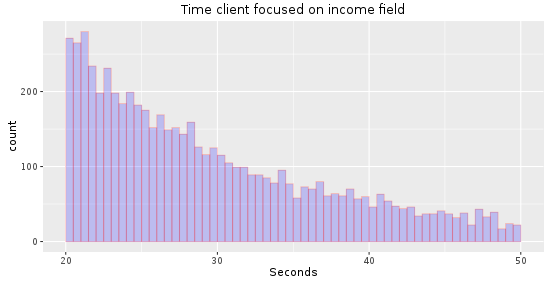
\includegraphics[scale=0.6]{Graphics/time_client_on_income.png}
    \caption{Histogram describing time a loan applicant focuses on the monthly income field, in seconds.}
    \label{fig:time-focused}
\end{figure}

Some values in Figure~\ref{fig:time-focused} are unusually large, possibly implying suspicious behavior when a would-be applicant tries to guess the income of a legitimate person.

An often used mathematical tool to demonstrate relationships between features is correlation analysis. The correlation plot (see figure: \ref{fig:corr-plott}) illustrates correlations between features related to the field for monthly income.  It shows near zero correlation between the focus time (observed above) and others, whereby for example the time past during changes and the count of tries to edit the particular field have an quite high correlation factor. However, some other features are moderately correlated. Visual exploration like this often guides a choice of data preprocessing to be applied and may reveal data quality issues.

\begin{figure}[h!]
    \centering
    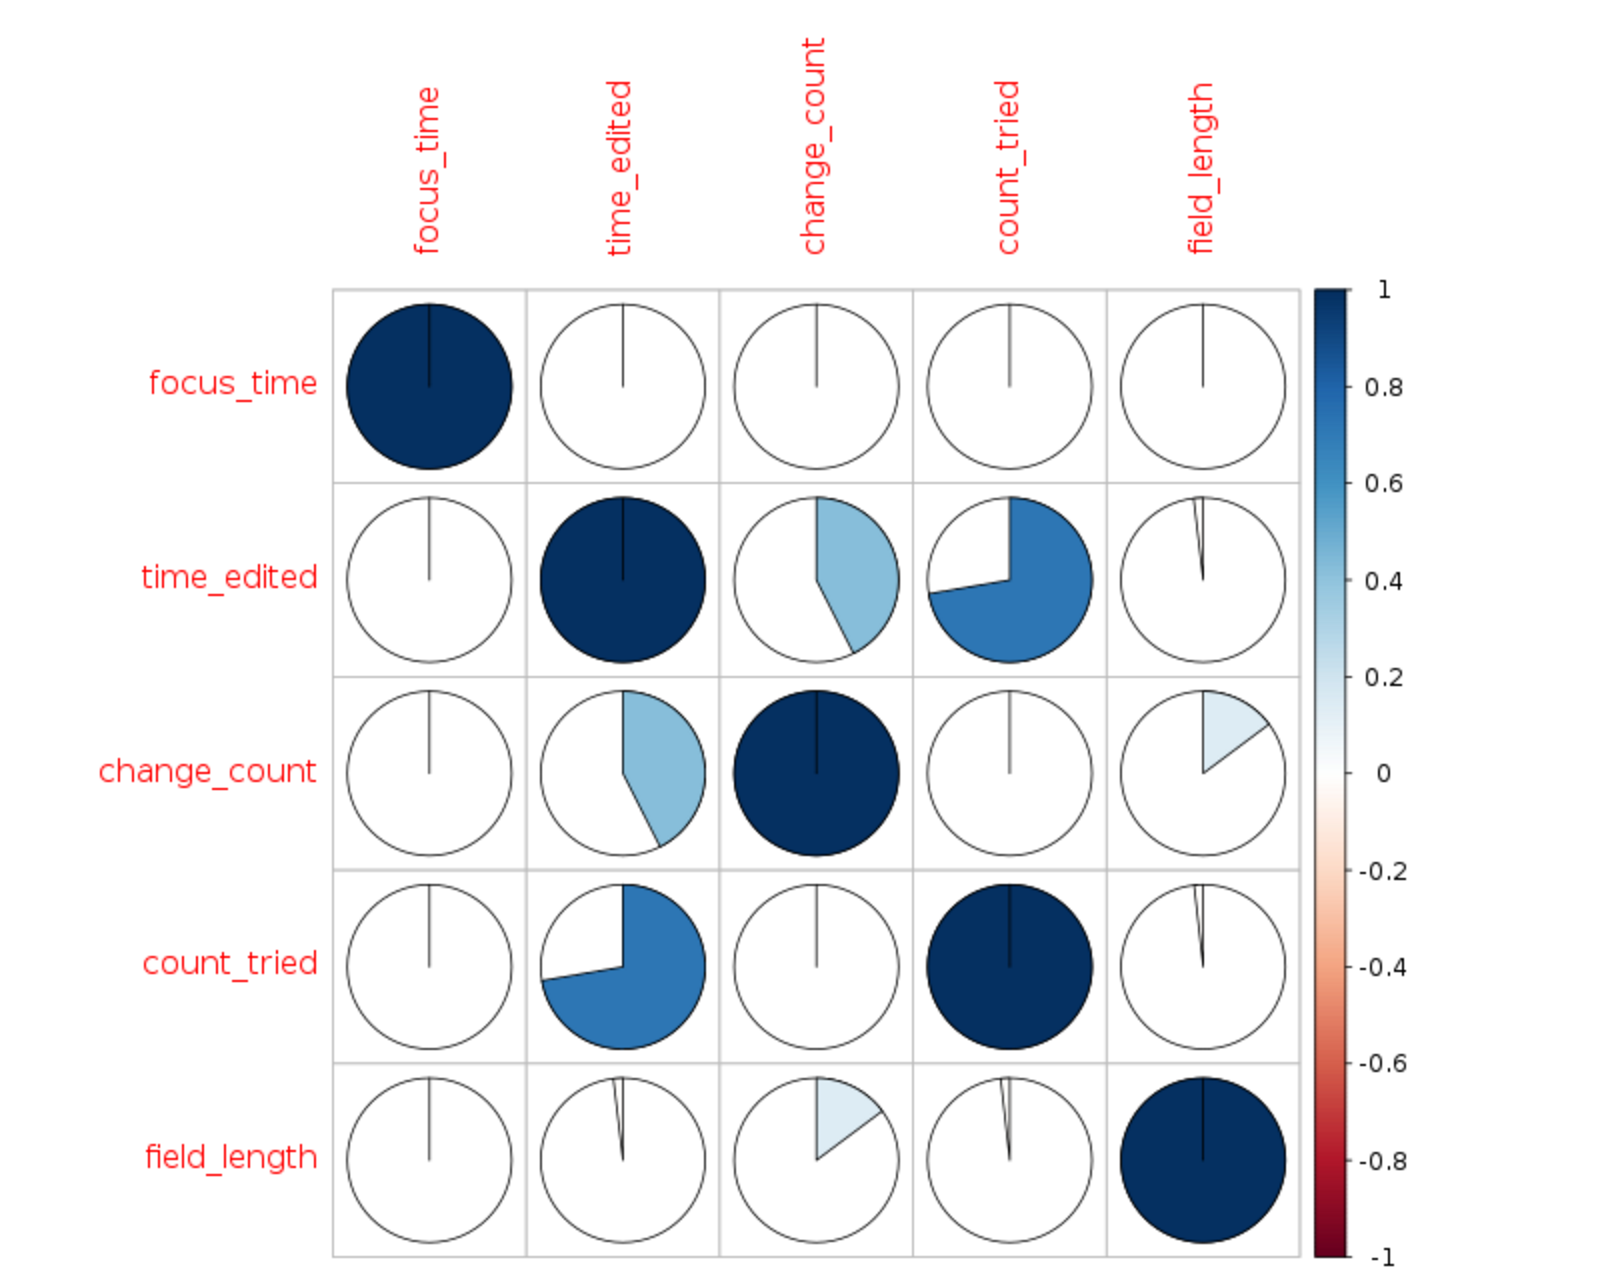
\includegraphics[scale=0.4]{Graphics/corr-plott.png}
    \caption{Pearson correlation plot over features that are describing behavior on the income field.} %footnote?
    \label{fig:corr-plott}
\end{figure}


\subsection{Data Quality (Missing Values)}\label{Ch:2:DataQuality}
\epigraph{The only really good solution to the missing data problem is not to have any. Statistical adjustments can never make up for sloppy research. }{Paul D. Allison, 2001}
\label{intro}

Lack of information or missing data in a given dataset is a common obstacle in field statistics and data mining. Below analysis is done in order to identify the amount of missing data. Table~\ref{tab:missings-over-all} presents a statistical summary of missing values in our source data.
 \begin{table}[h!]
  \begin{center}
    \caption{Summary of missing values in the entire data.}
    \label{tab:missings-over-all}
    \begin{tabular}{c|c|c|c|c|c}
    Min & 1st Quartile & Max & Median & Mean & 3rd Quartile \\
      \hline
     0\% & 8\% & 99\% & 31\% & 43\% & 77\% \\ 
     \hline 
    \end{tabular}
  \end{center}
\end{table}

It can be seen that there are some features containing all but missing values, and there are a plenty of features with about a half of values missing, implying that removal of rows with missing values is not an option because this would dramatically reduce the dataset size.

Since the lack of data is present, a deeper investigation is required. Missing data can have different types (in the context of statistical analysis). According to \cite{Allison:2007} there are three categories of missing data:

 \begin{itemize}
    \item \textbf{Missing Completely At Random (MCAR)} means that the probability of missing is unrelated to the feature itself or other features. 
    \item \textbf{Missing At Random (MAR)} addresses the missing in features that is unrelated to itself. For example, the probability of missing income may depends on the employment status, but does not depend on the income itself.
    \item \textbf{Not Missing At Random (NMAR)} eventuates when MAR is gone to be violated, ergo the probability of the missing depend on the particular value.
 \end{itemize}

Identifying the right category is important to select the correct treatment. However, classify the category of missing is not straight forward. An assumption about the membership is always based on observations on data and domain specific knowledge of data collection process.

Below the missing value analysis is broken down into the summaries grouped by feature type.

 \begin{table}[h!]
  \begin{center}
    \caption{Summary of missing values over logical data.}
    \label{tab:missings-over-logical}
    \begin{tabular}{c|c|c|c|c|c}
    Min & 1st Quartile & Max & Median & Mean & 3rd Quartile \\
      \hline
     5\% & 9\% & 99\% & 31\% & 43\% & 76\% \\ 
     \hline 
    \end{tabular}
  \end{center}
\end{table}
 
 \begin{table}[h!]
  \begin{center}
    \caption{Summary of missing values over numeric data.}
    \label{tab:missings-over-numeric}
    \begin{tabular}{c|c|c|c|c|c}
    Min & 1st Quartile & Max & Median & Mean & 3rd Quartile \\
      \hline
     0\% & 8\% & 99\% & 30\% & 41\% & 76\% \\ 
     \hline 
    \end{tabular}
  \end{center}
\end{table}
   

 \begin{table}[h!]
  \begin{center}
    \caption{Summary of missing values over categorical data.}
    \label{tab:missings-over-categorical}
    \begin{tabular}{c|c|c|c|c|c}
    Min & 1st Quartile & Max & Median & Mean & 3rd Quartile \\
      \hline
     0\% & 24\% & 99\% & 59\% & 58\% & 90\% \\ 
     \hline 
    \end{tabular}
  \end{center}
\end{table}

As follows from these tables, missing values are present in each group of features. The statistics for logical and numeric data are quite similar: This fact can lead to the assumption that causes of missing values may be related to a common factor(s), which, in turn, is indicative to the MAR category of missing values.

A common technique to check an assumption about the category of missing values is to inspect so called \textit{missing patterns}. It contributes to understanding whether groups of variables tend to be either all missing or all observed. Table~\ref{tab:variable-pattern-example} present a matrix, in which each row corresponds to a missing data pattern \textit{(1=observed, 0=missing).} 

\begin{table}[h!]
\centering
\caption{Missing pattern applied to four random variables.}
\label{tab:variable-pattern-example}
\begin{tabular}{lllll}
\textbf{No. of Cases} & V1 & V2 & V3 & V4 \\
901             & 1           & 1           & 1           & 1           \\
20              & 1           & 1           & 0           & 1           \\
4510            & 1           & 1           & 1           & 0           \\
2               & 0           & 1           & 1           & 1           \\
6               & 1           & 0           & 1           & 1           \\
87847           & 1           & 1           & 0           & 0           \\
9               & 0           & 1           & 1           & 0           \\
55              & 1           & 0           & 0           & 1           \\
6               & 1           & 0           & 1           & 0           \\
572             & 0           & 1           & 0           & 0           \\
716             & 1           & 0           & 0           & 0           \\
1307            & 0           & 0           & 0           & 0          
\end{tabular}
\end{table}

Furthermore, there is a visual investigation approach to identify missing patterns. Figure \ref{fig:missing-plot} presents two plots: The histogram shows the fraction of missing values and the box plot is the visualisation of missing patterns.

\begin{figure}[h!]
    \centering
    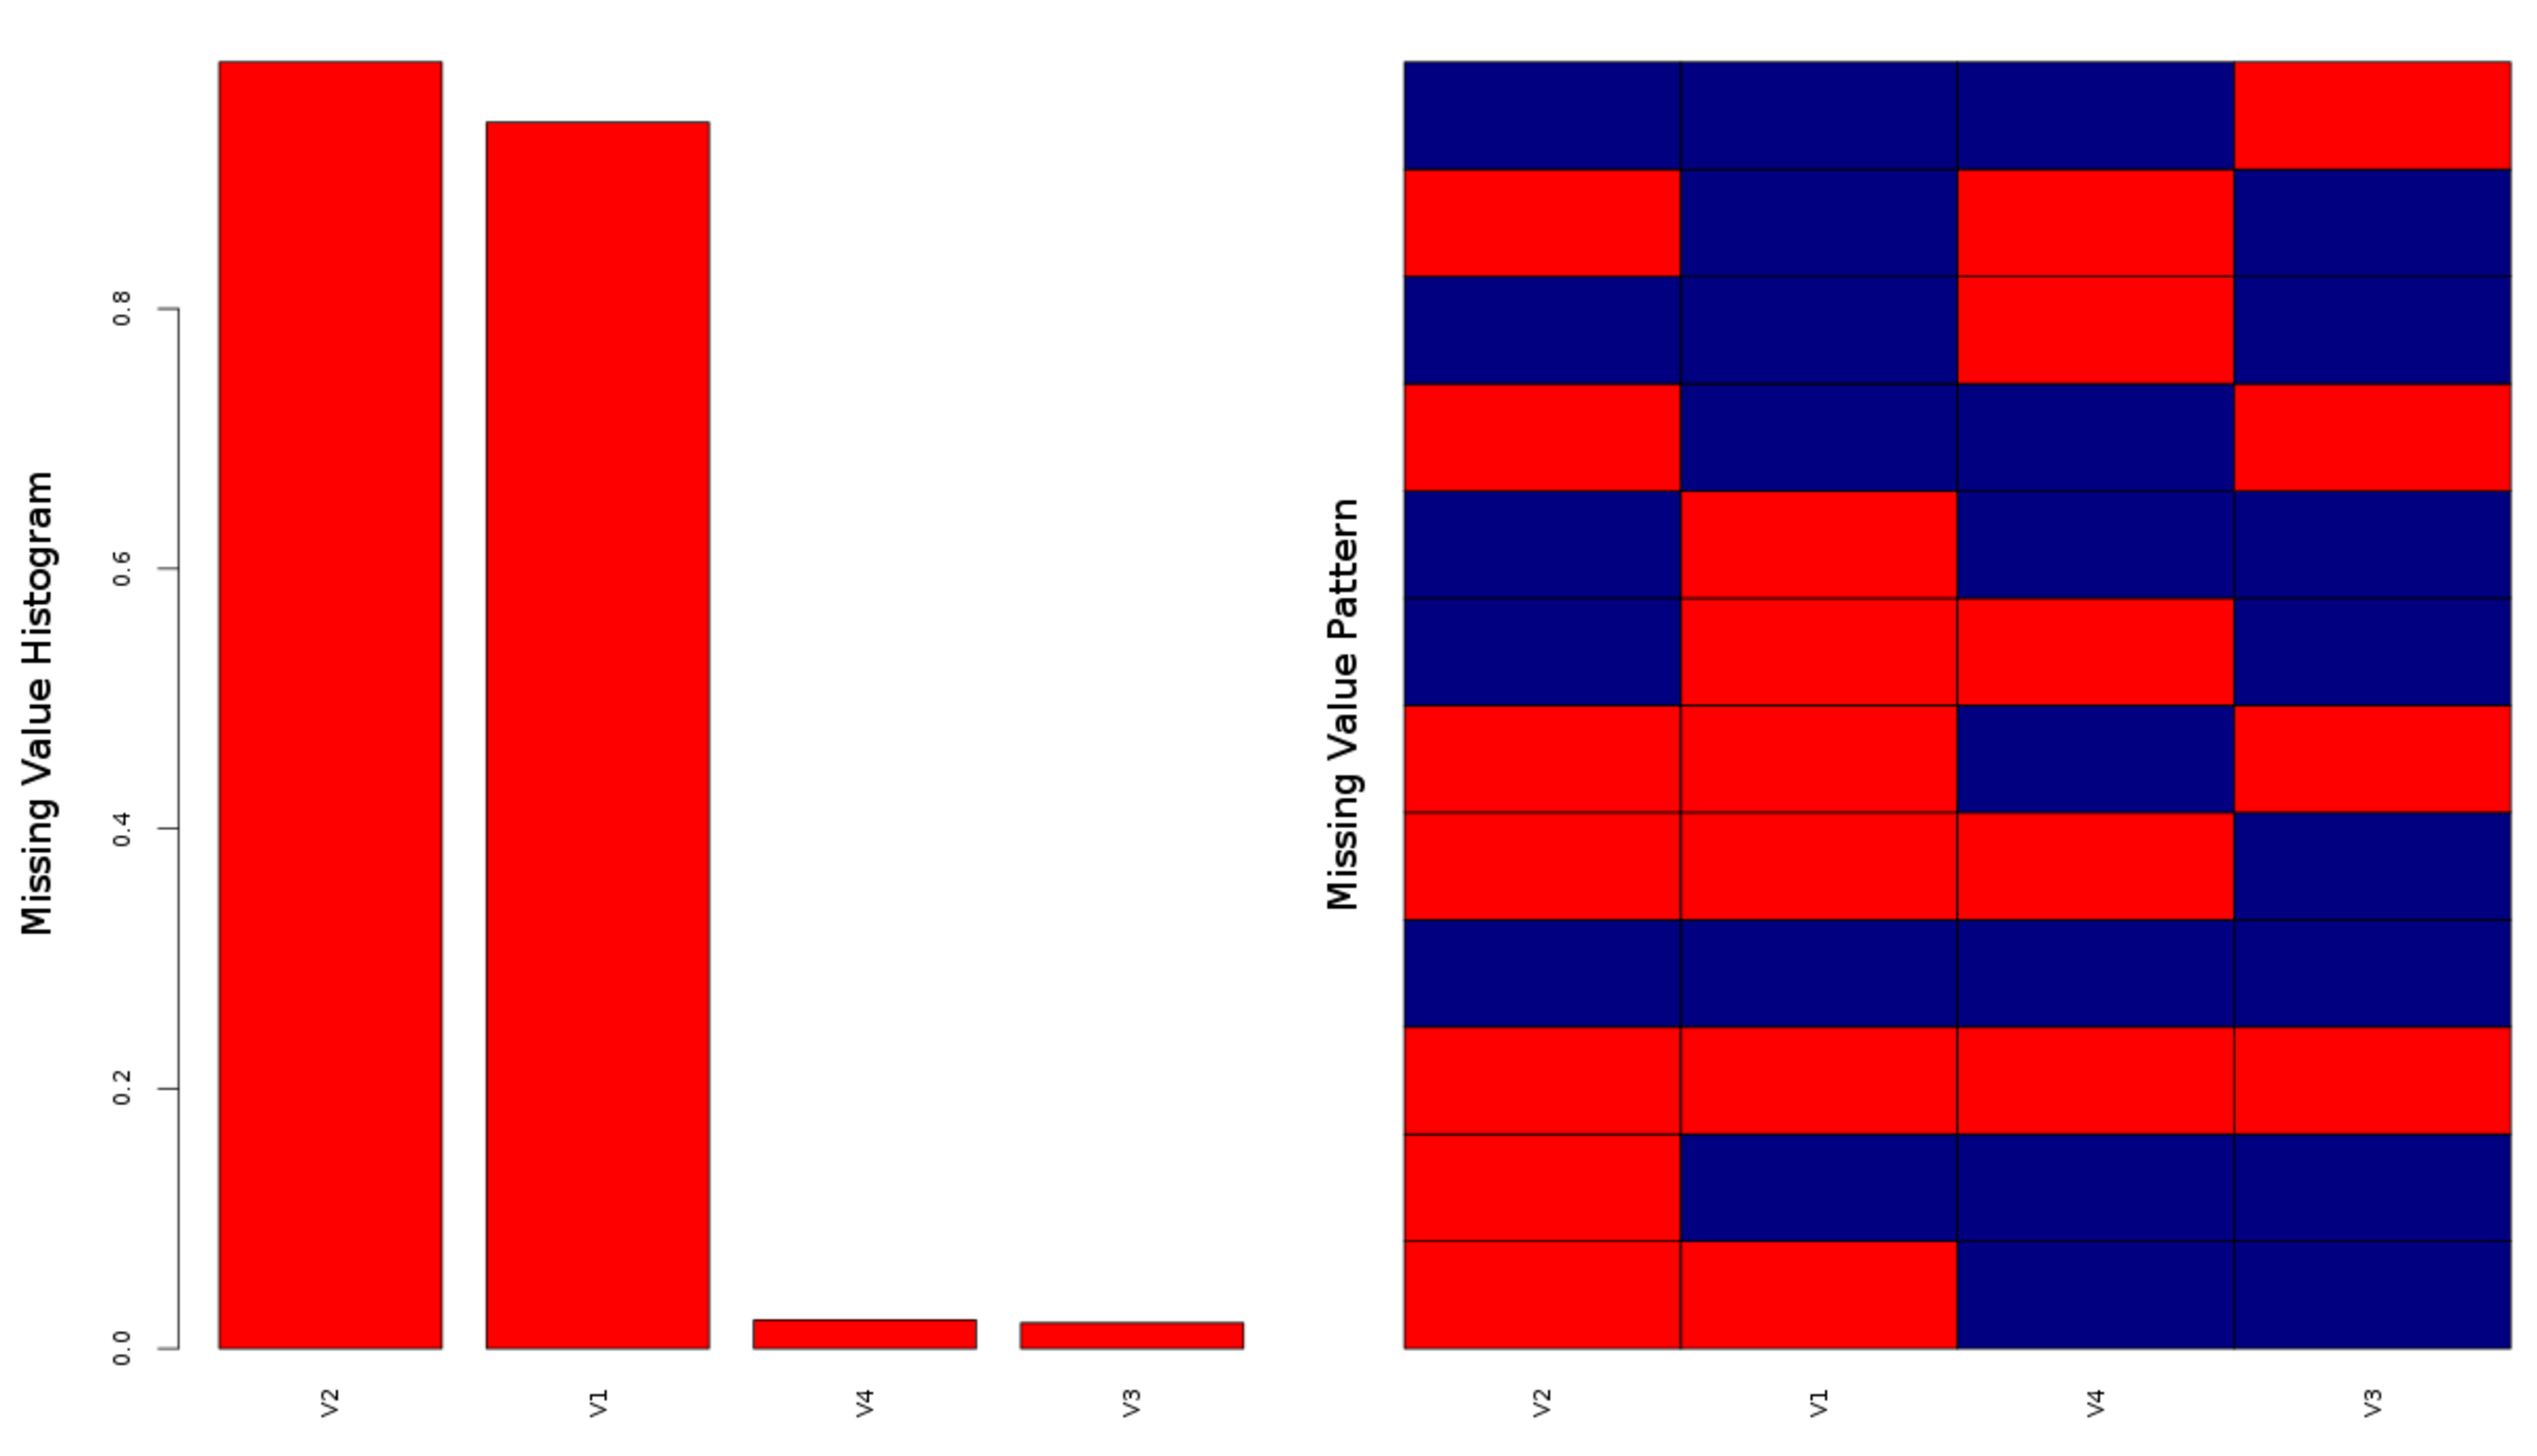
\includegraphics[scale=0.3]{Graphics/missing-pattern-plot.png}
    \caption{Missing pattern for the example in Table~\ref{tab:variable-pattern-example}.}
    \label{fig:missing-plot}
\end{figure}

Unfortunately, these analysis methods are only feasible for low-dimensional data. A pattern matrix describing all possible patterns in our data would obviously be hard to manage.

It is clear that more sophisticated techniques would produce valuable results in the case of categorization of the missingness. However, this topic is out of the scope of this thesis. However, the interested reader can check the work~\cite{Mohan;Pearl:2014}.

As last but not least, improving data collection practices should also be considered as powerful prevention of missing values. Possible causes of missing values can provide helpful information to increase data quality. 
Potential causes could be:
    \begin{itemize}
    
        \item Behavior data is describing several interactions with web form components, some of them are optional.
        
        \item Application data undergoes several processes before it is available for data analysis. The processing and data conversions related to these processes could be responsible for the loss of data.
        
        \item The credit application process was executed by a non-human but so-called script/bot \footnote{A bot (short for "robot") is a program that operates as an agent for a user or another program or simulates a human activity on the Internet. (http://searchsoa.techtarget.com/definition/bot)}. A bot obviously skips the most of the interactions a human would have to do during the application. 
    
        \item The particular operation system on the top of a loan application can be modified to block the gathering of information by the application system.
    \end{itemize}

\section{Preprocessing}\label{Ch:2:Preprocessing}
Based on the observations obtained through acquisition and exploration of our data, this section explains the necessary steps of data transformation to be made before building a predictive model.

\subsection{Categorical to Numeric Transformation}
\label{Ch:2:CTNT}
Many machine learning algorithms like those in Chapter~\ref{ch:3} cannot deal with other than numerical data types. Therefore logical and categorical data should be converted to a numeric representation before predictive modeling begins. 

The logical features are easy to convert: one value is replaced with 0 while the other with 1.

As for categorical features, the common approach is to replace each category level with a set of binary dummy variables, where the number of such variables is equal to the number of different levels.

Let us consider a categorical feature \textit{action} with the following levels: 

\[ \{ButtonClick, MouseClick, Other\} \]

For the sake of simplicity we consider a subset with only four instances as given in Table~\ref{tab:feature-categorical-rep}. 
\begin{table}[h!]
  \begin{center}
    \caption{Example of a categorical feature and its levels.}
    \label{tab:feature-categorical-rep}
    \begin{tabular}{c|c}
    instance & action \\
      \hline
     A & Other \\ 
     \hline 
       B & MouseClick \\ 
     \hline
       C & ButtonClick \\ 
     \hline
       D & Other \\ 
     \hline
    \end{tabular}
  \end{center}
\end{table}

Using binary dummy variables results in three additional features with a numerical value of either \(1\) or \(0\). Table~\ref{tab:feature-binarization} shows the result.

\clearpage


\begin{table}
  \begin{center}
    \caption{Result of the categorical-to-numeric transformation for the example in Table~\ref{tab:feature-categorical-rep}.}
    \label{tab:feature-binarization}
    \begin{tabular}{c|c|c|c|}
    instance & action.ButtonClick & action.MouseClick & action.Other \\
      \hline
     A & 0 & 0 & 1 \\ 
     \hline 
       B & 0 & 1 & 0 \\ 
     \hline
       C & 1 & 0 & 0 \\ 
     \hline
       D & 0 & 0 & 1 \\ 
     \hline
    \end{tabular}
  \end{center}
\end{table}

However, if the number of levels is too large, data dimensionality rapidly increases with each such a feature, thus contributing to noise and increased computation time.


\subsection{Missing Value Imputation}\label{Ch:2:MVI} 
This thesis will stick on different approaches for missing value imputation:

\begin{itemize}
    
        \item Mean imputation: each empty field will be replaced with a arithmetical average of a given distribution. However, this method is not robust, since it is largely influenced by outliers.
        
        \item Median imputation: where the empty fields are replaced by a value which represent a separation point of the higher half - from the lower half in a distribution. 
        
        \item Categorical imputation: an imputation technique for categorical data, where each empty value is imputed with a new invented category. For example an empty categorical feature \textit{place of work} will be imputed with the category \textit{other}. % HERE I NEED AN REASONING WHY I USE THIS PARTICULAR METHODOLOGY
        
      %  \item Extreme value imputation: involves imputing missing with an extreme high/low with respect to the underlying distribution. This technique follow the principal \textit{missing information is important information} so an extreme value underscore the weight of the feature in a particular case.
\end{itemize}



\subsection{Removing corrupted examples (acquisition error)}\label{Ch:2:RCD}
Since the process of data acquisition become more and more complex the chance to find a subset of flawed data points in the underlying dataset increase. Examples for corrupted data can be type errors (e.g a categorical value in a numeric field), extreme values (e.g a negative value in the field for monthly income) or missing values (separately discussed in Chapter ~\ref{Ch:2:DataQuality}). The causes are initially wrong input by user, erroneous type conversions or data transmission dropouts to name a few. 

A summary of the mean value (see Chapter ~ \ref{Ch:2:SSummary}) showed up the fact of existing negative numerical values in behavior data. However, behavior information can not be positive by definition\footnote{Behavior data considered in this Thesis can only have values >= 0, by definition.}.
Correcting such flawed entries efforts a detailed root-cause analysis. However, this is an engineering-heavy task and would go beyond the scope of this thesis. So the treatment in this Thesis will be to identify such kind of corruptions and exclude them from the dataset 


\subsection{Removing Zero- and Near-Zero Variance Features}\label{Ch:2:RNZVF}
Once all features become numeric, one can proceed with other transformations, namely a removal of features with zero and near zero variance as such features possess little or no power in discriminating classes of data. Think of the extreme example when all values for a given feature are the same, regardless a class label. The variance of such values is exactly zero and it is impossible to distinguish classes based on this feature alone.

Near-zero variance means that a feature takes very few unique values (relative to the number of instances) or has a large ratio of the first most common value to the second most common value.

Observations made by inspecting the data quality showed a significant number of missing values for some features, which implies that the data may likely contain features with zero and near-zero variance.

Although removal near-zero variance features seems to be desirable, there are situations where this might not be the case: For example, a native binary feature with a lot of zeroes and few ones could be a good discriminator between classes but the near-zero variance check could possibly remove it.

\subsection{Principle Component Analysis (PCA)}\label{Ch:2:PCA} 
Principle Component Analysis is one of the main methods to reduce dimensionality, first introduced by Karl Pearson \cite{Pearson:1901}. The main idea behind PCA is to reduce the number of features through a linear transformation aiming at finding directions of maximal data variance. Given a large number of features in our dataset, doing PCA is a reasonable preprocessing step. PCA also makes features uncorrelated, which is an attractive characteristic when there is suspicion of correlation among the original features.

Formally, the goal of PCA is to map data instances from higher- to lower-dimensional space:

\[ x \in X \in {\rm I\!R}^n \textrm{ to } z \in Z \in {\rm I\!R}^k \]
\[ \textrm{where } k \leq n \]

The classical approach is first to compute a \(n \times n \) covariance matrix (an beside effect of that is centering)\footnote{Centering is a technique where an constant value (often the mean value) is gonna be subtracted from every value of a variable.}, where each element is the covariance between two features:

\[ \Sigma = \frac{1}{m}\sum_{i = 1}^{n}(x^i)(x^i)^T\]
\[ \textrm{where }(x^i) \textit{ is a } (1 \times n) \textrm{ vector and } (x^i)^T \textrm{is a } (n \times 1) \textrm{ vector.}\]

Eigenvectors and eigenvalues of this matrix are then computed. Eigenvectors determine the directions of a new feature space, corresponding to the maximum data variance and their eigenvalues explain the variance of the data.

There are several methods to compute the eigenvectors.
In this thesis the method the \textit{Singular Value Decomposition} (SVD) will be used thus is an proved and numeric stable approach \cite{wall2003svd,zouht04}.  

Applying SVD to the covariance matrix, yields:

\[ [U,S,V] = SVD(\Sigma)\]
\[ \textrm{where  } U \in  {\rm I\!R}^{n \times n} \textrm{ Matrix representing the eigenvectors.}  \]

Sorting eigenvalues in descending order of magnitude and selecting the \( k \) eigenvectors corresponding to the top \( k \) eigenvalues, results in \( U' \in   {\rm I\!R}^{n \times k}\) matrix.

Transforming the original data \( X \) to a new space is done by

\[ Z = X U'^ T \]

Although PCA is widely used for dimensionality reduction, the latter causes certain information loss. The extent of such loss needs to be kept in mind when PCA is followed by data classification. 